\documentclass[11pt,titlepage]{article}
%\usepackage{eufrak,epsfig}
\usepackage{epsfig}
\usepackage{graphicx}
\usepackage{latexsym}
\usepackage{amssymb}
\usepackage{amsmath,amscd}
\usepackage{multirow} 
\usepackage{array}
\usepackage{caption}
\usepackage {subfig}
\usepackage{color}
\usepackage{natbib}
\usepackage{rotating}
\usepackage{graphicx,lscape}
\usepackage{hyperref}
\usepackage{indentfirst}
\usepackage{tikz}
\usepackage{pgfplots}
\usepackage[margin=3.1cm]{geometry}
\usepackage{kotex}
\long\def\comment#1{} 

%\nofiles
\newcommand{\rb}[1]{\raisebox{-.5em}[0pt]{#1}}
\renewcommand{\baselinestretch}{1.7}
\renewcommand{\mid}{\, | \ , }
\newcommand{\eighth}{{\textstyle \frac{1}{8}}}

\newcommand{\by}{\mbox{\boldmath $y$}}
\newcommand{\bx}{\mbox{\boldmath $x$}}
\newcommand{\bd}{\mbox{\boldmath $d$}}
\newcommand{\bv}{\mbox{\boldmath $v$}}
\newcommand{\bu}{\mbox{\boldmath $u$}}
\newcommand{\bl}{\mbox{\boldmath $\ell$}}
\newcommand{\bW}{\mbox{\boldmath $W$}}
\newcommand{\bX}{\mbox{\boldmath $X$}}
\newcommand{\bY}{\mbox{\boldmath $Y$}}
\newcommand{\bA}{\mbox{\boldmath $A$}}
\newcommand{\bV}{\mbox{\boldmath $V$}}
\newcommand{\bL}{\mbox{\boldmath $L$}}
\newcommand{\bdm}{\begin{displaymath}}
\newcommand{\edm}{\end{displaymath}}
\newcommand{\bbeta}{\mbox{\boldmath $\beta$}}
\newcommand{\btheta}{\mbox{\boldmath $\theta$}}
\newcommand{\btt}{\mbox{\boldmath $\theta$}}
\newcommand{\bep}{\mbox{\boldmath $\epsilon$}}

\newcommand{\balpha}{\mbox{\boldmath $\alpha$}}
\newcommand{\bxi}{\mbox{\boldmath $\xi$}}
\newcommand{\bXi}{\mbox{\boldmath $\Xi$}}
\newcommand{\bmu}{\mbox{\boldmath $\mu$}}
\newcommand{\bgamma}{\mbox{\boldmath $\gamma$}}

\newcommand{\bphi}{\mbox{\boldmath $\phi$}}
\newcommand{\bpsi}{\mbox{\boldmath $\psi$}}
\newcommand{\C}{{\rm Cov}}

\newcommand{\bld}[1]{\mbox{\boldmath $#1$}}
\newcommand{\bmmu}{\bld \mu}
\newcommand{\bbf}{\bld f}
\newcommand{\bbe}{\bld e}
\newcommand{\bbg}{\bld g}
\newcommand{\bbx}{\bld x}
\newcommand{\bbz}{\bld z}
\newcommand{\cC}{{\cal C}}
\newcommand{\cB}{{\cal B}}
\newcommand{\cH}{{\cal H}}

\renewcommand{\baselinestretch}{1.8}
\setlength\arraycolsep{2pt}
\linespread{1.5}

\title{\bf Prediction of Extremal Precipitation: Use of Quantile Regression Forests
\medskip
}

\author{
	Seoncheol Park\footnote{Graduate Student, Department of Statistics, Seoul National
		University, 1 Gwanak-ro, Gwanak-gu, Seoul 08826, Korea. 
		pscstat@gmail.com}, Junhyeon Kwon\footnote{Graduate Student, Department of Statistics, Seoul National
		University, 1 Gwanak-ro, Gwanak-gu, Seoul 08826, Korea. 
		junhyeonkwon@gmail.com}, Joonpyo Kim\footnote{Graduate Student, Department of Statistics, Seoul National
		University, 1 Gwanak-ro, Gwanak-gu, Seoul 08826, Korea. 
		joonpyokim@snu.ac.kr} and Hee-Seok Oh\footnote{Professor, Department of Statistics, Seoul National
		University, 1 Gwanak-ro, Gwanak-gu, Seoul 08826, Korea. 
		heeseok.oh@gmail.com} \\
	Department of Statistics\\
	Seoul National University\\
	Seoul 08826, Korea\\
	\\
}

%\date{Draft: version of \today}
\date{\today}

\begin{document}
	
	\maketitle
	
	\begin{abstract}
		
		This paper suggests a random forest method for spatio-temporal extreme value prediction of precipitation data. The proposed method is based on a quantile regression forests method, a kind of data mining method, improves other methods, tree and bagging. To represent monthly correlation of the data, we adopt circular transformed predictors. Throughout real data analysis, the empirical prediction performance of the proposed method is better than other methods and the prediction score of the proposed method is competitable with other team's method.
		%Real data analysis show that the use of circular transformed predictors are useful to improve prediction performance.
		
		% to predict the extremal spatio-temporal prediction of precipitation data. We also suggest the use of circular transform to represent the monthly correlation. The results are competitible.
		
		\vskip 7mm
		
		\noindent {\it Keywords}: Quantile regression forests, Circular transform, Ensemble, Spatio-temporal extremes.
		
	\end{abstract}

	\section{Introduction}
	앙상블 기법은 그동안 많은 발전이 있었다. 그 중에서도 랜덤 포레스트는 성공적인 앙상블 예측 기법 중 하나다. 한편, \citep{Meinshausen2006}은 quantile regression forests를 개발해 평균 예측만 사용되는 random forests를 분위수 예측에 사용할 수 있게 하였다. 분위수 회귀 포레스트를 가지고 높은 quantile을 예측하려는 시도는 여럿 있었다. Quantile regression forests는 기상 자료 분석에 많이 사용되어왔다.  \citep{Taillardat2016}은 quantile regression forest 기반 예측 방법을 프랑스 surface temperature와 wind speed 예측에 사용하고 기존 방법보다 좋은 예측 결과를 얻었다. \citep{Aznarte2017}는 스페인 마드리드에서 기상요소들이 extreme $\text{NO}_{2}$ 농도에 미치는 영향을 알아보기 위해 quantile regression forests를 사용했다.
	
	한편, Circular-linear or circular-circular regression methods have been used in various area, especially in the environmental study. There are some previous studies using those kind of regressions. \citep{Johnson1978} explained special joint distributions when linear and circular variables are in explanatory variables and they have special marginal distributions. After then they applied it to the regression problem with air pollution as a response variable, temperature as a linear predictor and wind direction as a circular predictor.. \citep{Jammalamadaka2006}는 sine, cosine 변환을 한 month, wind direction을 predictor로써 포함하여 이들이 ozone level에 미치는 영향을 circular-circular regression으로 분석하였다.
	본 연구에서는 이러한 사전연구들에 힌트를 얻어 네덜란드의 각 관측장소별 월 별 20-year return level에 해당하는 극단 강수량 예측을 QRF에 기반한 방법들로 예측해 보고 그 결과를 비교해 보았다. 월(month) 간 correlation을 반영하기 위해 circular-transformed predictor variable을 고려하였고 그 결과 예측 성능을 높일 수 있었다. 2장에서는 자료에 대한 소개 및 결측치 제거 방법에 대해 말하였다. 3장에서는 본 논문에서 사용한 방법론들을 소개하였다. 4장에서는 모형 구축 및 제안한 모형의 성능을 제시하였고 그 결과를 비교하였다. 마지막으로 5장에서는 본 연구의 한계점과 앞으로 나아가야 할 점들을 제시하였다.
	
	\section{Data Description and Missing Data Treatment}
	
	\begin{figure}
		\centering
		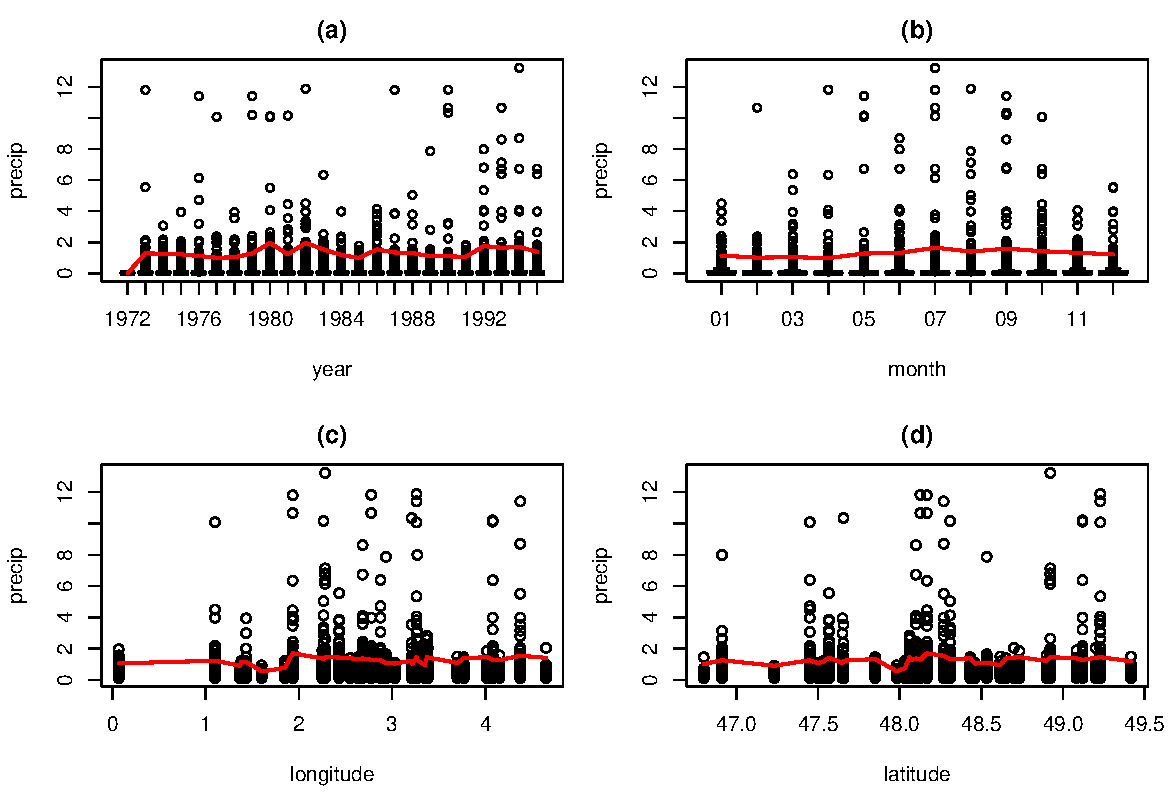
\includegraphics[scale=0.75]{Scatter3.pdf}
		%\vspace{-7mm}
		\caption{Scatter plot between precipitation and year (top left), month (top right), longitude (bottom left) and latitude (bottom right). Red lines mean empircal 0.998 conditional quantile.}
		\label{fig:scatter}
	\end{figure}
	
	In this paper, we can consider five explanatory variables candidates, \texttt{year}, \texttt{month}, \texttt{date},  \texttt{longitude} and \texttt{latitude}, etc. Figure \ref{fig:scatter} shows scatter plots between predictor variable candidates and response variables. \

	From the explanatory analysis, we know some characteristics of the data. First, we have no strong linear trend between year and precipitation. That means we can' find significant increasing or decreasing trend of extreme precipitation across year. In this paper, we assume that year doesn't effect for the extreme precipitation in future 20 years. Second, we also find the relationship between longitue or latitude and extreme precipitation is nonlinear. In this paper, we assume that there exists some local increasing or decreasing behavior of extreme precipitation through longitude or latitude. Finally, there is a little seasonal trend of extreme precipitation. Extreme precipitaion is high in summer, low in spring.
	
	\begin{figure}[h!]
		\centering
		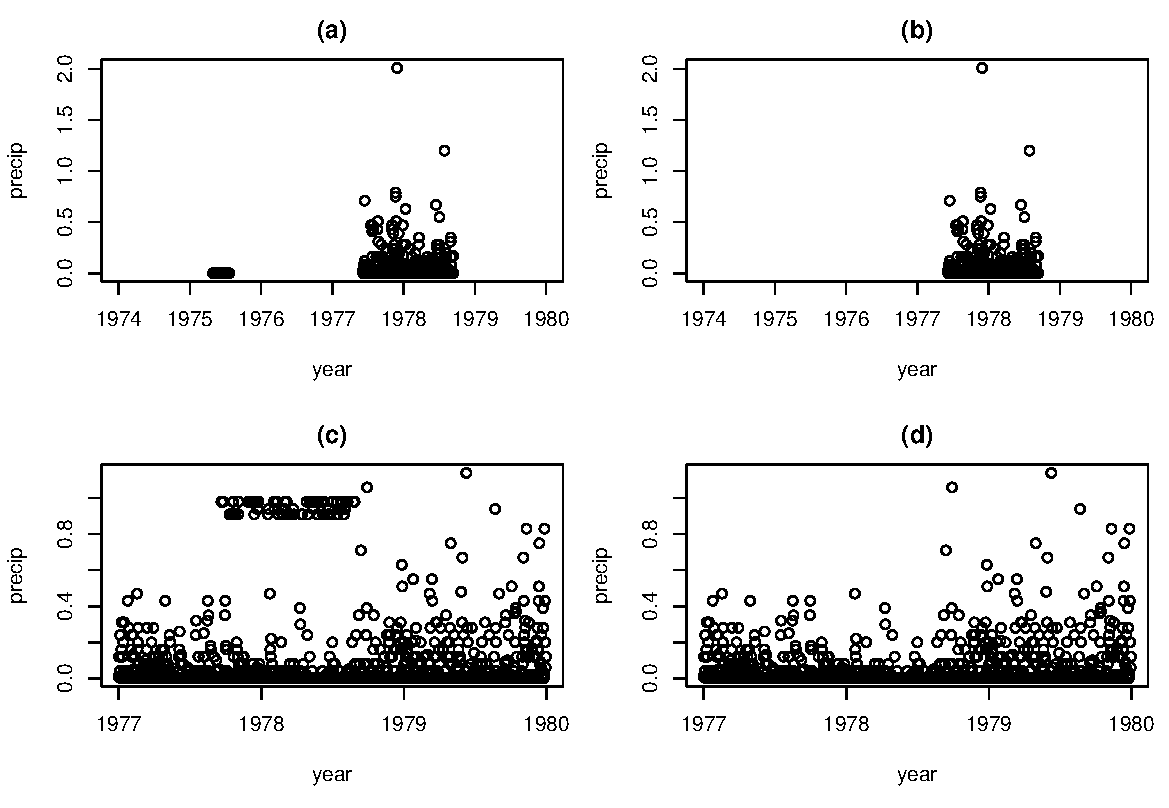
\includegraphics[scale=0.75]{Missing.pdf}
		\caption{Illusration xample of data treatment. Since (a) original time series at station 31 have some zero values in 1975, (b) we delete those values. (c) In station 4, time series have some strange values from 1977 to 1979, therefore (d) we delete those values.}
		\label{fig:DTM}
	\end{figure}
	
	On the other hand, most of the time series have many missing values, as in Figure \ref{fig:DTM}. That means, it is hard to apply time-series based approach to this data. As a result of explanatory data analysis, we could observe that some stations have too many missing values. Therefore, traditional time-series based apporoach is hard to use in this data. A circular transform is used to express the monthly correlation.
	
	
	
	\section{Methods}
	
	\subsection{Regression Tree}
	
	Decision tree is a kind of data mining methods and first suggested by \citep{Breiman1984}. When response variable is numeric, then it is called 'regression tree'. In this paper, we focus on regression tree. %We introduce some notations for explanations.
	
	Suppose there are $n$ observations, let the set of data $\mathbf{Z}_{i}$, $\mathcal{D}_{n}=\{ \mathbf{Z}_{1},\dots , \mathbf{Z}_{n} \}$ be a learning set. The data $\mathbf{Z}_{i}$ is $\mathbf{Z}_{i}=(Y_{i},\mathbf{X}_{i})$, where $Y_{i}, i=1,\ldots,n$ be dependent variables and $\mathbf{X}_{i}=(X_{i,1},\ldots, X_{i,p})$ be $p$-dimensional independent variables. In this paper, we assume that there is a non-linear, complex relationship between dependent variables and independent varibles. That means, we assume there is a non-linear, complex function $f$ such that
	$$y_{i}=f(\mathbf{x}_{i})+\epsilon_{i},\qquad{ i=1,\ldots,n.}$$
	
	Let $\mathcal{X}$ be the covariate space. The main idea of regression tree is making adequate partitions of $\mathcal{X}$ by diving $\mathcal{X}$ into $L$ disjoint sets $\mathcal{R}_{1}, \ldots, \mathcal{R}_{L}$ to have homogeneous $Y_{i}$ values in each partition. After then, regression tree fits a piecewise-constant prediction at each partition.
	

	
	For further explanation, we introduce some notations in \citep{Breiman2001}. The leaf of a tree $l(\mathbf{x})$ is a rectangular subspace of $\mathcal{X}$. 
	Then, the prediction of a single tree %$T(\boldsymbol{\theta})$ 
	for a new data point $\mathbf{X}=\mathbf{x}$ is obtained by averaging over the observed values in leaf $l(x)$. Let the weight vector $w_{i}(\mathbf{x})$ %given by a positive constant if observation $\mathbf{X}_{i}$ is part of leaf $l(\mathbf{x},\theta)$ and 0 if it is not. The weights sum to one, and thus,
	represents whether the observation $\mathbf{X}_{i}$ is part of leaf $l(\mathbf{x})$ or not,
	\begin{equation}\label{eq:treeweight}
	w_{i}(\mathbf{x})=\frac{1_{\{ \mathbf{X}_{i} \in R_{l(\mathbf{x})} \}}}{\# \{ j: \mathbf{X}_{j} \in R_{l(\mathbf{x})} \}}.
	\end{equation}
	The prediction of a single tree, given covariance $\mathbf{X}=\mathbf{x}$, is then the weighted average of the original observations $Y_{i},i=1,\ldots,n$,
	%$$\text{single tree: } \hat{E}(Y|\mathbf{X}=\mathbf{x})=\sum_{i=1}^{n}w_{i}(\mathbf{x},\theta)Y_{i}.$$
	\begin{equation}\label{eq:treepred}
	\hat{f}(\mathbf{X})=\hat{E}(Y|\mathbf{X}=\mathbf{x})=\sum_{i=1}^{n}w_{i}(\mathbf{x})Y_{i}.
	\end{equation}
	%In this view, decision tree can be considered as a local constant model. 
	
	Regression tree has some benefits. It is easy to interpret, can do explanatory variable selection implicitly. It also needs only a few tuning parameters, so the computation consideration is simple. It doesn't need any formal distributional assumptions, so it can also model  the nonlinear relationship between explanatory variables and response variable. %It doesn't affect the scale of variables. So, we don't need to normalize the data. 
	%It is computationally simple and quick to fit, even for large problems. Regression tree doesn't need formal distributional assumptions (non-parametric). It is easy to interpret when the size of tree is small.
	However, tree method also has some disadvantages. First, trees usually have high variance due to its greedy split process. That means small change in training data can give very different splits. Second, since the tree estimation is not smooth, it is not good when underlying function is smooth. %Due to it hiercrachical and greed estimation process, tree method is not robust.
	
	\subsection{Random Forests}
	
	To overcome the disadvantages of regression tree, ensemble methods are suggested. \citep{Breiman1996} suggested a new method called Bagging. The main idea of bagging is averaging many trees to bootstrap-resampled versions of the training data to reduce the variance of regression trees.
	
	Furthermore, \citep{Breiman2001} suggested random forests. In addition to bagging, random forests uses a random subset of predictor variables for covariate space split selection to make more decorrelated trees. It makes an improvement of the prediction performace of random forest compared to bagging.
	
	Based on the notations of \citep{Meinshausen2006}, we summarize random forest algorithms. Suppose we generate $k$ single trees for model construction. Then, for $t=1$ to $k$, we repeat following three steps:
	
	\begin{enumerate}
		\item Draw a bootstrap sample from the training data.
		\item Select $m$ $(m < p)$ variables at random and call them $\boldsymbol{\theta}_{t}$.
		\item Grow a single tree $T(\boldsymbol{\theta}_{t})$.
	\end{enumerate}

	Then, the prediction of conditional mean $E(Y|\mathbf{X}=\mathbf{x})$ is given by an average prediction of $k$ single trees, %each constructed with an independent and identically distributed (i.i.d.) vector $\boldsymbol{\theta}_{t}$,
	\begin{equation}\label{eq:conexpectation}
	\hat{f}(\mathbf{X})=\hat{E}(Y|\mathbf{X}=\mathbf{x})=\sum_{i=1}^{n}w_{i}(\mathbf{x})Y_{i},
	\end{equation}
	where
	\begin{equation}\label{eq:singletreepredw}
	w_{i}(\mathbf{x})=\frac{\sum_{t=1}^{k}w_{i}(\mathbf{x},\boldsymbol{\theta}_{t})}{k}, \qquad{w_{i}(\mathbf{x},\boldsymbol{\theta})=\frac{1_{\{ 	\mathbf{X}_{i} \in R_{l(\mathbf{x},\boldsymbol{\theta})} \}}}{\# \{ j: \mathbf{X}_{j} \in R_{l(\mathbf{x},\boldsymbol{\theta})} \}} }.
	\end{equation}
	%meaning of weight: QRF 논문에서 weight의 의미는 i-th tranining example이 leaf x에 얼마나 자주 떨어지는 지 그 정도를 나타내는 것 
	
	For each tree grown on a bootstrap sample, the error rate for observations left out of the bootstrap sample is monitored. \citep{Breiman2001} called it as  “out-of-bag (oob)” error rate. In the notation of \citep{Gregorutti2017}, we consider an estimator based on the observation of a out-of-bag sample $\bar{\mathcal{D}}$
	\begin{equation}
	\hat{R}(\hat{f}, \bar{\mathcal{D}})=\frac{1}{|\bar{\mathcal{D}}|}\sum_{i:(\mathbf{X}_{i},Y_{i})\in\bar{\mathcal{D}}}^{|\bar{\mathcal{D}}|}(Y_{i}-\hat{f}(\mathbf{X}_{i}))^{2}
	\end{equation}
	
	Then we can get the empirical permutation performance of the variable $X_{j}$,
	\begin{equation}
	\hat{I}(X_{j})=\frac{1}{k}\sum_{t=1}^{k}[\hat{R}(\hat{f}_{t}, \bar{\mathcal{D}}_{n}^{tj})-\hat{R}(\hat{f}_{t},\bar{\mathcal{D}}_{n}^{t}) ], \qquad{j=1,\ldots, p}
	\end{equation}
	which can be used to measure the importance of each predictor variable.
	
%	\subsubsection{Variable Importance in Random Forests}
	
	%(out of bag case, variable importance에 대한 설명, Reo Breiman의 설명)
	
	%In every tree grown in the forest, put down the oob cases and count the number of votes cast for the correct class. Now randomly permute the values of variable m in the oob cases and put these cases down the tree. Subtract the number of votes for the correct class in the variable-m-permuted oob data from the number of votes for the correct class in the untouched oob data. The average of this number over all trees in the forest is the raw importance score for variable m.
	
	%If the values of this score from tree to tree are independent, then the standard error can be computed by a standard computation. The correlations of these scores between trees have been computed for a number of data sets and proved to be quite low, therefore we compute standard errors in the classical way, divide the raw score by its standard error to get a z-score, ands assign a significance level to the z-score assuming normality.
	
	%If the number of variables is very large, forests can be run once with all the variables, then run again using only the most important variables from the first run.
	
	%For each case, consider all the trees for which it is oob. Subtract the percentage of votes for the correct class in the variable-m-permuted oob data from the percentage of votes for the correct class in the untouched oob data. This is the local importance score for variable m for this case, and is used in the graphics program RAFT.
	
	%(가장 결과가 좋은 방법의 variable importance를 boxplot의 형태로 출력하기)
	
	%( random forest에서는 variable importance plot을 제공해 주므로 variable importance의 boxplot을 같이 제시)
	
	\subsection{Quantile Regression Forests}
	
	Sometimes we have an interest about conditional quantile, not conditional mean.  \citep{Meinshausen2006} tried to do random forest for conditional quantiles, names as quantile regression forests (QRF). The conditional distribution function of $Y$ given $\mathbf{X}=\mathbf{x}$ is given by
	\begin{equation}
	F(y|\mathbf{X}=\mathbf{x})=P(Y\leq y| \mathbf{X}=\mathbf{x})=E(1_{\{Y\leq y\}}|\mathbf{X}=\mathbf{x}).
	\end{equation}
	
	\citep{Meinshausen2006} showed that these $w_{i}$ in (\ref{eq:singletreepredw}) can also be used to estimate the conditional distribution function, $\hat{F}(y|\mathbf{X}=\mathbf{x})$ by plugging in $1_{\{Y\leq y\}}$ instead of $Y$ in equation (\ref{eq:conexpectation}):
	\begin{equation}\label{eq:qrfprediction}
	\hat{F}(y|\mathbf{X}=\mathbf{x})=\sum_{i=1}^{n}w_{i}(\mathbf{x})1_{\{Y_{i}\leq y\}}.
	\end{equation}
	In QRF, they uses same weight $w_{i}(\mathbf{x})$ as in random forests. Therefore, QRF only changes the equation (\ref{eq:conexpectation}) to (\ref{eq:qrfprediction}). The corresponding conditional quantile of level $\tau$ is
	\begin{equation}
	\hat{Q}_{\tau}(y|\mathbf{x})=\inf \{ y:\hat{F}_{Y|\mathbf{X}}(y|\mathbf{x})\geq \tau \}.
	\end{equation}
	%Note that, \citep{Meinshausen2006} does not use check-function based loss minimization methods. Instead, he uses a plug-in estimator to get the conditional quantiles.
	
	\subsection{Generalized Quantile Regression Forests}
	
	\citep{Athey2016} suggest a new method called generalized random forests (GRF). The main differences between quantile regression forest and generalized quantile random forests are twofolds. First, they used esimating equation to solve various loss minimization problem. Second, they changed splitting scheme according to score function.
	
	Suppose that we want to estimate a quantity, $\theta(\mathbf{x})$. In this challenge, $\theta(\mathbf{x})$ is the $\tau$-th conditional quantile function, i.e., $\theta(\mathbf{x})=Q_{\tau}(y|\mathbf{x})$.  GRF solve the following local estimating equation:
	\begin{equation}\label{eq:momentcondsample}
	E[\psi_{Q_{\tau} (\mathbf{x})}(Y_{i})|\mathbf{X}_{i}=\mathbf{x}]=0, \qquad{\forall \mathbf{x}\in\mathcal{X},}
	\end{equation}
	where $\psi(\cdot)$ is a appropriate score function. In quantile regression forests, $\psi_{Q_{\tau}(\mathbf{x})}(Y_{i})=\tau\mathbf{1}(\{ Y_{i}>Q_{\tau}(\mathbf{x})\})- (1-\tau)\mathbf{1}(\{ Y_{i}\leq Q_{\tau}(\mathbf{x}) \})$. In this paper, we called it generalized quantile regression forests (GQRF). %\citep{Athey2016} refered that one popular approach of estimating $Q_{\tau}(\mathbf{x})$ is to apply similarity weights $w_{i}(x)$ which measures the relavance between $i$-th data and $Q_{\tau}(\mathbf{x})$. It coincide with the weight of quantile regression forests. We can fit $Q_{\tau}(\mathbf{x})$ using the empirical version of (\ref{eq:momentcondsample}),
	%\begin{equation}\label{eq:empiricalmomentcondsample}
	%(\hat{Q}_{\tau}(\mathbf{x}))\in\arg\min_{Q_{\tau}(\mathbf{x})}\{\| \sum_{i=1}^{n}w_{i}(\mathbf{x})\psi_{Q_{\tau}(\mathbf{x})}(Y_{i}) \|_{2} \}.
	%\end{equation}
	%where we can use forest-based weights (\ref{eq:singletreepredw}).
	
	\citep{Athey2016} suggest a new spliting method based on above estimation equation using gradient-based approximation. Let the parent node be $P \subset \mathcal{X}$. Suppose $\hat{Q}_{\tau,P}(\mathbf{x})$ is computed by an empirical version of (\ref{eq:momentcondsample}),
	\begin{equation}
	\hat{Q}_{\tau,P}(\mathcal{D}_{n})\in\arg\min_{Q_{\tau}(\mathbf{x})}\{ \| \sum_{\{ i:(\mathbf{X}_{i},Y_{i})\in \mathcal{D}_{n}, X_{i}\in P \}} \psi_{Q_{\tau}}(Y_{i})  \|_{2} \}
	\end{equation}
	
	The main ingredient of tree is dividing a parent leaf $P$ into two child leaves, $H_{1}$ and $H_{2}$ with an suitable criteria. %Let $\hat{Q}_{\tau,P}$ is the prediction value of parent node and  
	%Quantile regression forests uses a standard CART regressin splitting rule in \citep{Breiman1984}. Unlike it, 
%	
	
	%그러나 위 식으로부터 직접 split selection을 하는 경우 계산량이 많아, \citep{Athey2016}은 $\hat{Q}_{\tau,C_{1}}, \hat{\theta}_{\tau,C_{2}}$를 gradient-based approximation해서 구성하여 최적화하는 gradient tree algorithm을 제안하였다. 이 알고리즘은 우리가 $\hat{Q}_{\tau,P}$를 알고 있다고 가정할 때 , $\hat{Q}_{\tau, C}\approx \tilde{Q}_{\tau,C}$로 근사하는 것이다.
	%\begin{equation}
	%\tilde{Q}_{\tau, C}=\hat{Q}_{\tau, P}+\frac{1}{ \{ i:X_{i}\in C \} }\sum_{ \{ i : X_{i}\in C\} }\rho_{i},
	%\end{equation}
	%where $\rho_{i}$ is a pseudo-outcome. In GQRF, \citep{Athey2016} showed that it becomes
	%\begin{equation}\label{eq:labelingstep}
	%%\rho_{i}=\xi^{T}A_{P}^{-1}\psi_{\hat{\theta}_{P}, \hat{\nu}_{P}}(O_{i})\in\mathbb{R}.
	%\rho_{i}=\mathbf{1}(\{ Y_{i}>\hat{Q}_{\tau,P} \}),
	%\end{equation}
	%In generalized quantile regression forests, 
	%\citep{Athey2016} said the meaning of \ref{eq:labelingstep} is that the gradient-based quantile regression trees simply try to separate observations that fall above the $q$-th quantile of the parent from those below it.
	%To do this, GRF used a gradient-based approximation algorithm:
	%new algorithm, named "gradient tree algorithm". It finds $C_{1}$ and $C_{2}$ maximize criterion $\tilde{\Delta}(C_{1},C_{2})$ using gradient-based approximations for $\hat{Q}_{\tau, C_{1}}$ and $\hat{Q}_{\tau, C_{2}}$. 
	
	\begin{enumerate}
		\item First, GQRF gets pseudo-outcomes $\rho_{i}=\mathbf{1}(\{ Y_{i}>\hat{Q}_{\tau,P} \})$ using the $q$-the quantile of the parent $P$, $\hat{Q}_{\tau,P}$ to .
		\item Next, GQRF runs a regression split on the pseudo-outcomes $\rho_{i}$. Specially, GQRF splits $P$ into two axis-aligned children $H_{1}$ and $H_{2}$ to maximize the criterion
		\begin{equation}\label{eq:regressionstep}
		\tilde{\Delta}(H_{1},H_{2})=\sum_{j=1}^{2}\frac{-1}{ | \{ i : X_{i}\in H_{j} \} | }\Big(\sum_{\{ i \: X_{i}\in H_{j} \}}\rho_{i}\Big)^{2}.
		\end{equation}
		\item Then, GQRF computes a gradient-based approximation of $q$-th quantile of the child nodes $\hat{Q}_{\tau, H}$ by
		\begin{equation}\label{eq:gradientapprox}
		\tilde{Q}_{\tau, H}=\hat{Q}_{\tau, P}+\frac{1}{|\{ i: X_{i}\in C \}|}\sum_{\{ i:X_{i}\in H \} }\rho_{i}, \qquad{H \in \{H_{1}, H_{2} \}.}
		\end{equation}
		\item GQRF recursively continues above steps.
	\end{enumerate}
	
	Note that \citep{Athey2016} don't claim their GQRF is alway better than quantile regression forests. Empirically, GQRF would produce smoother sample paths than QRF. Splitting rule of GRF is specially sensitive to quantile shifts in a way that regression splits are not. However, traditional mean-based regression trees are sensive to shifts of $E(Y|\mathbf{X})$.
	
	\subsection{Circular Transform}
	
	In this paper, we consider three types of circular transform of month. One of the natural way is that in Figure \ref{fig:circular1}, we places a month in the clock. 12월을 (1,0) 즉 시계로 얘기하면 3시 방향에 놓고 counter-clockwise 방향으로 달들을 배치한 다음 이들의 \texttt{cosine}, \texttt{sine} 값을 설명변수로 사용하였고 이들 두 개의 변수들을 \texttt{cosmonth}, \texttt{sinmonth}로 부르기로 한다. We called circular-transformed month variable as \texttt{cosmonth} and \texttt{sinmonth}.
	
	We consider monthly-circular transformed data (Figure \ref{fig:circular1}). In monthly-circular transformed data, we put 12 (cosine, sine) value at each month.
	
	We also consider finer-scale circular transforms. In Figure \ref{fig:circular2}는 Figure \ref{fig:circular1}를 좀 더 세분화하여 한 달을 early, late part로 나눈 후 circular transform을 취한 것이다. 이렇게 생성된 변수들을 \texttt{cosmonth*}, \texttt{sinmonth*}라고 부르기로 한다. Figure \ref{fig:circular3}는 한 달을 early, middle, late part 셋으로 세분화 한 후 circular transform을 취한 것이다. 이렇게 생성된 변수들을 \texttt{cosmonth**}, \texttt{sinmonth**}라고 부르기로 한다.
	
	원래 날은 연속된 형태의 자료이나 부득이하게 12개의 class로 나누어 계산되었는데, 이것을 좀 더 continuous하게 만들고자 하는 의도가 있었다. 그리고 여러 모형의 예측값을 가중평균으로 나타내 안정적인 예측 결과를 얻고자 하는 목표가 있었다. 그러나 완전한 continuous한 변수로 보기에는 자료의 수가 너무 적었기에 상순 중순 하순 보다 더 세밀하게 나누는 작업은 고려하지 않았다.
	
	%이렇게 달을 세분해서 고려할 경우, 특정 달의 상순과 하순, 또는 특정 달의 상순과 중순 하순의 극단 강수량이 큰 차이를 보일 때, 그리고 특정 달의 하순과 그 다음 달의 상순 사이에 강한 상관관계를 갖고 있다고 가정할 때 예측에 더 도움이 될 수 있을 것이다. 
	
	Further, when there is an irrgularity of maximum within the month, it may be useful to adopt finer division. (Figure \ref{fig:circular2} and Figure \ref{fig:circular3}). It may also solve the discrete problem of original monthly-circular transform. 2번째 모형에서는 한 달의 상순, 하순의 0.998 quantile을 예측 한 후 이들의 평균을 취했으며, 3번째 모형에서는 한 달의 상순, 중순, 하순의 0.998 quantile을 예측한 후 이들의 평균을 취하였다.
	
	We divide a month into two parts: early and late (cosmonth* and sinmonth*), or three parts: early, middle and late (cosmonth** and sinmonth**). 
	
	Model 2 and 3 gives a better prediction result when there is a strong relationship (달이 바뀔 시.) .
	\begin{figure}
		\centering
		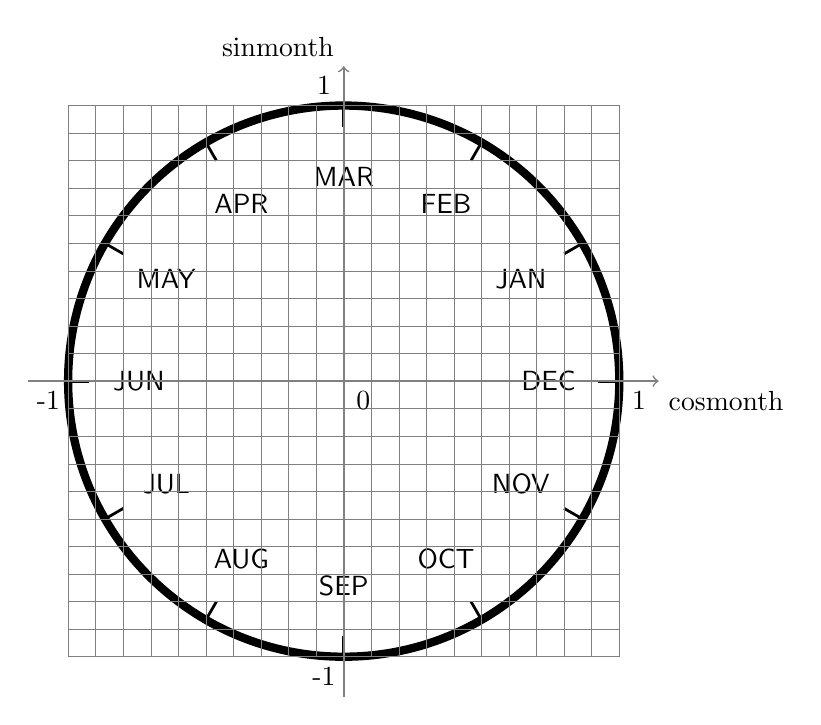
\begin{tikzpicture}[line cap=rect,line width=3pt]
		%\begin{axis}[
		%axis lines = center,
		%axis line style={latex-latex},
		%clip=false]
		%\end{axis}
		\filldraw [fill=white] (0,0) circle [radius=3.5cm];
		\foreach \angle [count=\xi] in {30,60,...,360}
		{
			\draw[line width=1pt] (\angle:3.25cm) -- (\angle:3.5cm);
			%\node[font=\large] at (\angle:1.75cm) {\textsf{\xi}};
		}
		\node[font=\normalsize] at (30:2.6cm) {\textsf{JAN}};
		\node[font=\normalsize] at (60:2.6cm) {\textsf{FEB}};
		\node[font=\normalsize] at (90:2.6cm) {\textsf{MAR}};
		\node[font=\normalsize] at (120:2.6cm) {\textsf{APR}};
		\node[font=\normalsize] at (150:2.6cm) {\textsf{MAY}};
		\node[font=\normalsize] at (180:2.6cm) {\textsf{JUN}};
		\node[font=\normalsize] at (210:2.6cm) {\textsf{JUL}};
		\node[font=\normalsize] at (240:2.6cm) {\textsf{AUG}};
		\node[font=\normalsize] at (270:2.6cm) {\textsf{SEP}};
		\node[font=\normalsize] at (300:2.6cm) {\textsf{OCT}};
		\node[font=\normalsize] at (330:2.6cm) {\textsf{NOV}};
		\node[font=\normalsize] at (360:2.6cm) {\textsf{DEC}};
		%\foreach \angle in {0,90,180,270}
		%\draw[line width=2pt] (\angle:1.6cm) -- (\angle:2cm);
		%\draw (0,0) -- (120:0.8cm);
		%\draw (0,0) -- (90:1cm);
		
		\draw[semithick, gray,->] (-4,0) -- (4,0) node[anchor=north west, black] {cosmonth};
		\draw[semithick, gray,->] (0,-4) -- (0,4) node[anchor=south east, black] {sinmonth};;
		\draw[step=3.5cm,gray,very thin] (-3.501,-3.501) grid (3.5,3.5);
		\draw[step=0.35cm,gray,very thin] (-3.501,-3.501) grid (3.5,3.5);
		
		\node at (-3.75,-0.25) {-1};
		\node at (3.75,-0.25) {1};
		\node at (0.25,-0.25) {0};
		\node at (-0.25, 3.75) {1};
		\node at (-0.25,-3.75) {-1};
		\end{tikzpicture}
		\caption{Circular transform of type 1.} \label{fig:circular1}
	\end{figure}
	\begin{figure}
		\centering
		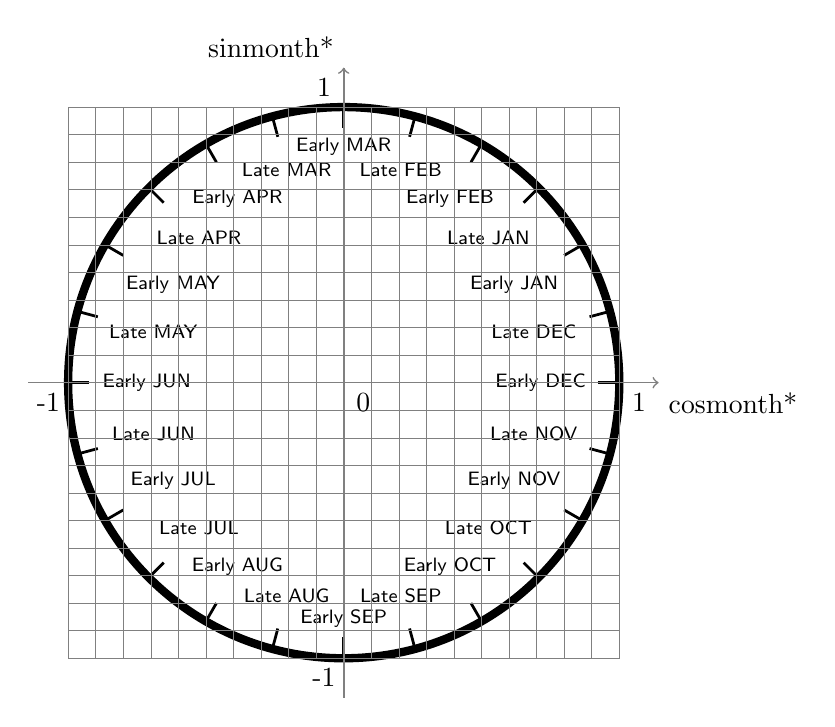
\begin{tikzpicture}[line cap=rect,line width=3pt]
		\filldraw [fill=white] (0,0) circle [radius=3.5cm];
		\foreach \angle [count=\xi] in {30,45,60,...,360,375}
		{
			\draw[line width=1pt] (\angle:3.25cm) -- (\angle:3.5cm);
			%\node[font=\large] at (\angle:1.36cm) {\textsf{\xi}};
		}
		\node[font=\scriptsize] at (30:2.5cm) {\textsf{Early JAN}};
		\node[font=\scriptsize] at (45:2.6cm) {\textsf{Late JAN}};
		\node[font=\scriptsize] at (60:2.7cm) {\textsf{Early FEB}};
		\node[font=\scriptsize] at (75:2.8cm) {\textsf{Late FEB}};
		\node[font=\scriptsize] at (90:3.0cm) {\textsf{Early MAR}};
		\node[font=\scriptsize] at (105:2.8cm) {\textsf{Late MAR}};
		\node[font=\scriptsize] at (120:2.7cm) {\textsf{Early APR}};
		\node[font=\scriptsize] at (135:2.6cm) {\textsf{Late APR}};
		\node[font=\scriptsize] at (150:2.5cm) {\textsf{Early MAY}};
		\node[font=\scriptsize] at (165:2.5cm) {\textsf{Late MAY}};
		\node[font=\scriptsize] at (180:2.5cm) {\textsf{Early JUN}};
		\node[font=\scriptsize] at (195:2.5cm) {\textsf{Late JUN}};
		\node[font=\scriptsize] at (210:2.5cm) {\textsf{Early JUL}};
		\node[font=\scriptsize] at (225:2.6cm) {\textsf{Late JUL}};
		\node[font=\scriptsize] at (240:2.7cm) {\textsf{Early AUG}};
		\node[font=\scriptsize] at (255:2.8cm) {\textsf{Late AUG}};
		\node[font=\scriptsize] at (270:3.0cm) {\textsf{Early SEP}};
		\node[font=\scriptsize] at (285:2.8cm) {\textsf{Late SEP}};
		\node[font=\scriptsize] at (300:2.7cm) {\textsf{Early OCT}};
		\node[font=\scriptsize] at (315:2.6cm) {\textsf{Late OCT}};
		\node[font=\scriptsize] at (330:2.5cm) {\textsf{Early NOV}};
		\node[font=\scriptsize] at (345:2.5cm) {\textsf{Late NOV}};
		\node[font=\scriptsize] at (360:2.5cm) {\textsf{Early DEC}};
		\node[font=\scriptsize] at (375:2.5cm) {\textsf{Late DEC}};
		
		
		\draw[semithick, gray,->] (-4,0) -- (4,0) node[anchor=north west, black] {cosmonth*};
		\draw[semithick, gray,->] (0,-4) -- (0,4) node[anchor=south east, black] {sinmonth*};
		\draw[step=3.5cm,gray,very thin] (-3.501,-3.501) grid (3.5,3.5);
		\draw[step=0.35cm,gray,very thin] (-3.501,-3.501) grid (3.5,3.5);
		
		\node at (-3.75,-0.25) {-1};
		\node at (3.75,-0.25) {1};
		\node at (0.25,-0.25) {0};
		\node at (-0.25, 3.75) {1};
		\node at (-0.25,-3.75) {-1};
		\end{tikzpicture}
		\caption{Circular transform of type 2.} \label{fig:circular2}
	\end{figure}
	
		\begin{figure}
		\centering
		
		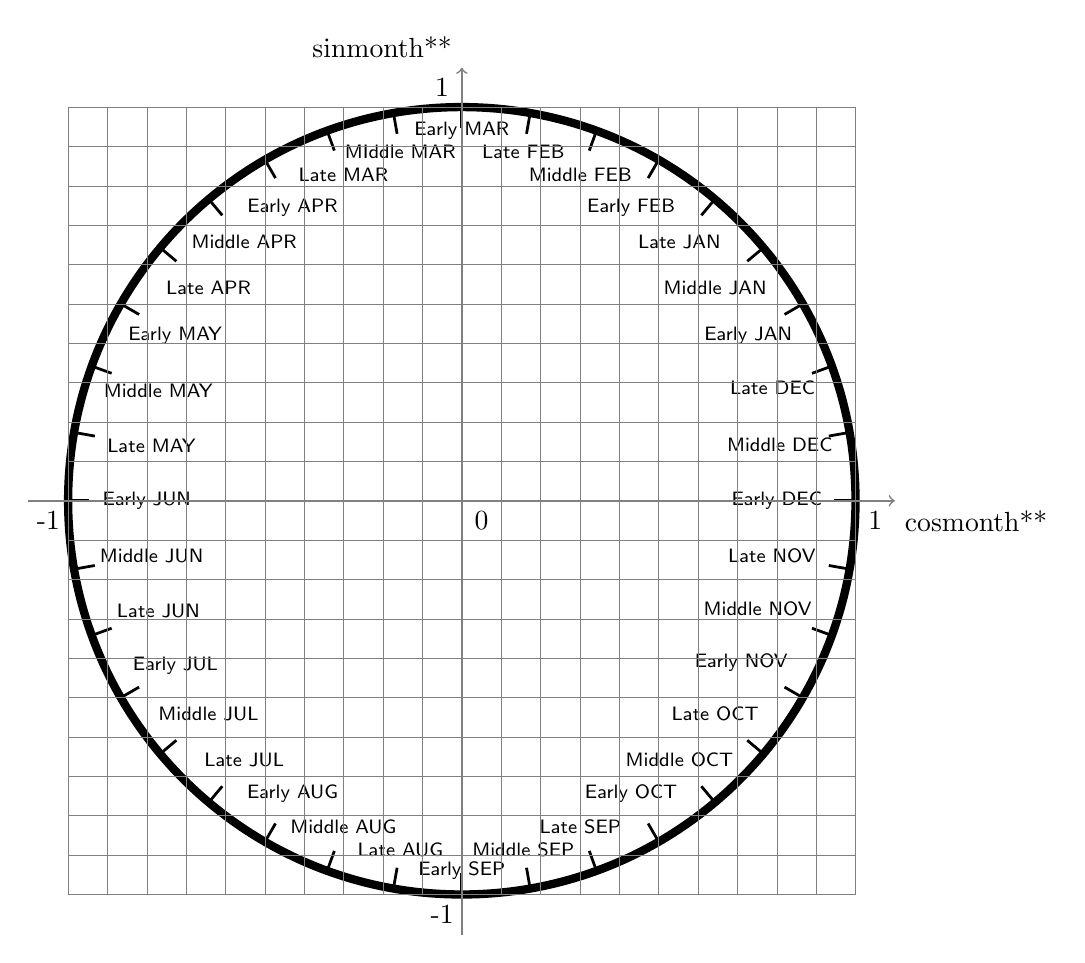
\begin{tikzpicture}[line cap=rect,line width=3pt]
		\filldraw [fill=white] (0,0) circle [radius=5cm];
		\foreach \angle [count=\xi] in {30,40,50,...,380}
		{
			\draw[line width=1pt] (\angle:4.75cm) -- (\angle:5cm);
			%\node[font=\large] at (\angle:1.36cm) {\textsf{\xi}};
		}
		\node[font=\scriptsize] at (30:4.2cm) {\textsf{Early JAN}};
		\node[font=\scriptsize] at (40:4.2cm) {\textsf{Middle JAN}};
		\node[font=\scriptsize] at (50:4.3cm) {\textsf{Late JAN}};
		\node[font=\scriptsize] at (60:4.3cm) {\textsf{Early FEB}};
		\node[font=\scriptsize] at (70:4.4cm) {\textsf{Middle FEB}};
		\node[font=\scriptsize] at (80:4.5cm) {\textsf{Late FEB}};
		\node[font=\scriptsize] at (90:4.7cm) {\textsf{Early MAR}};
		\node[font=\scriptsize] at (100:4.5cm) {\textsf{MIddle MAR}};
		\node[font=\scriptsize] at (110:4.4cm) {\textsf{Late MAR}};
		\node[font=\scriptsize] at (120:4.3cm) {\textsf{Early APR}};
		\node[font=\scriptsize] at (130:4.3cm) {\textsf{Middle APR}};
		\node[font=\scriptsize] at (140:4.2cm) {\textsf{Late APR}};
		\node[font=\scriptsize] at (150:4.2cm) {\textsf{Early MAY}};
		\node[font=\scriptsize] at (160:4.1cm) {\textsf{Middle MAY}};
		\node[font=\scriptsize] at (170:4.0cm) {\textsf{Late MAY}};
		\node[font=\scriptsize] at (180:4.0cm) {\textsf{Early JUN}};
		\node[font=\scriptsize] at (190:4.0cm) {\textsf{Middle JUN}};
		\node[font=\scriptsize] at (200:4.1cm) {\textsf{Late JUN}};
		\node[font=\scriptsize] at (210:4.2cm) {\textsf{Early JUL}};
		\node[font=\scriptsize] at (220:4.2cm) {\textsf{Middle JUL}};
		\node[font=\scriptsize] at (230:4.3cm) {\textsf{Late JUL}};
		\node[font=\scriptsize] at (240:4.3cm) {\textsf{Early AUG}};
		\node[font=\scriptsize] at (250:4.4cm) {\textsf{Middle AUG}};
		\node[font=\scriptsize] at (260:4.5cm) {\textsf{Late AUG}};
		\node[font=\scriptsize] at (270:4.7cm) {\textsf{Early SEP}};
		\node[font=\scriptsize] at (280:4.5cm) {\textsf{Middle SEP}};
		\node[font=\scriptsize] at (290:4.4cm) {\textsf{Late SEP}};
		\node[font=\scriptsize] at (300:4.3cm) {\textsf{Early OCT}};
		\node[font=\scriptsize] at (310:4.3cm) {\textsf{Middle OCT}};
		\node[font=\scriptsize] at (320:4.2cm) {\textsf{Late OCT}};
		\node[font=\scriptsize] at (330:4.1cm) {\textsf{Early NOV}};
		\node[font=\scriptsize] at (340:4.0cm) {\textsf{Middle NOV}};
		\node[font=\scriptsize] at (350:4.0cm) {\textsf{Late NOV}};
		\node[font=\scriptsize] at (360:4.0cm) {\textsf{Early DEC}};
		\node[font=\scriptsize] at (370:4.1cm) {\textsf{Middle DEC}};
		\node[font=\scriptsize] at (380:4.2cm) {\textsf{Late DEC}};
		
		\draw[semithick, gray,->] (-5.5,0) -- (5.5,0) node[anchor=north west, black] {cosmonth**};
		\draw[semithick, gray,->] (0,-5.5) -- (0,5.5) node[anchor=south east, black] {sinmonth**};;
		\draw[step=5cm,gray,very thin] (-5.001,-5.001) grid (5,5);
		\draw[step=0.5cm,gray,very thin] (-5.001,-5.001) grid (5,5);
		
		\node at (-5.25,-0.25) {-1};
		\node at (5.25,-0.25) {1};
		\node at (0.25,-0.25) {0};
		\node at (-0.25, 5.25) {1};
		\node at (-0.25,-5.25) {-1};
		\end{tikzpicture}
		\caption{Circular transform of type 3.} \label{fig:circular3}
	\end{figure}

	\section{Models and Results}
	
	\subsection{Models}
	
	We consider several models:
	
	\begin{enumerate}
		\item For preliminary results of challenge, we adopted circular-transformed quantile regression forests (CQRF) with precipitation(\texttt{precip}) as a response variable, \texttt{longitudes}, \texttt{latitudes}, (\texttt{cosmonth}) and (\texttt{sinmonth}) are predictor variables. %The preliminary result is one realization after excluding results having too many high prediction values. %Unfortunately, we did not save the original seed. %Among several new attempts after your final announcement mail, we could find that set.seed(5213) gives similar result. We save the source code for the algorithm in ``QRF(middle).R".
		$$\text{CQRF: } \texttt{precip }\sim \texttt{lon + lat + cosmonth + sinmonth.}\qquad{\text{(CQRF)}}$$
		
		\item For final results of challenge, we used an emsemble of circular-transformed quantile regression forests (ECQRF) with data-adaptive weight using inverse of losses. The idea is based on using more detailed division of the circular transform to consider more time information. 
		
		제시한 예측 모형은 3개 모형의 앙상블이다. 첫 번째 모형은 CQRF를 그대로 사용한 것이다. 두 번째 모형과 세 번째 모형은 \texttt{cosmonth}, \texttt{sinmonth}를 좀 더 세분화한 예측변수를 사용한 CQRF 모형을 사용하였다.
				
		Then, we perform circular transform and quantile regression forests:
		$$\text{Model 1: }\texttt{precip }\sim \texttt{lon + lat + cosmonth + sinmonth.}\qquad{\text{(CQRF)}}$$
		$$\text{Model 2: }\texttt{precip }\sim \texttt{lon + lat + cosmonth* + sinmonth*.}$$
		$$\text{Model 3: }\texttt{precip }\sim \texttt{lon + lat + cosmonth** + sinmonth**.}$$
		
		ECQRF is the weighted average of three models. To decide the weights, we compute the inverse of losses. To do this, we divide the given data into training (80$\%$) and validation (20$\%$) set and compute the empirical losses on validation set.  Given station $j, j=1,\ldots, 40$ and month $k, k=1,\ldots, 12$  sum of empirical losses on validation set is
		
		$$S_{j,k}(\hat{Q}_{\text{Model i},j,k} )= \sum_{\text{day t of the validation period in month k}} l(P_{j,t},\hat{Q}_{\text{Model i},j,k}), \qquad{i=1,2,3.}$$
		
		Then the weight matrix is
		
		$$W_{\text{Model i}}=
		\begin{bmatrix}
		w_{j,k}^{i}
		\end{bmatrix}
		, \qquad{w_{j,k}^{i} = \frac{1/S_{j,k}(\hat{Q}_{\text{Model i},j,k})}{\sum_{i=1}^{3}1/S_{j,k}(\hat{Q}_{\text{Model i},j,k})} .}$$
		If there is no available training data for some $(j,k)$ we use the average weight of whole losses, i.e., $w_{j,k}^{i} = \frac{1/\sum_{j,k}S_{j,k}(\hat{Q}_{\text{Model i},j,k})}{\sum_{i=1}^{3}1/\sum_{j,k}S_{j,k}(\hat{Q}_{\text{Model i},j,k})} .$
		
		Final ECQRF prediction is
		
		$$\text{ECQRF: }W_{\text{Model 1}}\circ \hat{Q}_{\text{Model 1}}+W_{\text{Model 2}}\circ \hat{Q}_{\text{Model 2}}+W_{\text{Model 3}}\circ \hat{Q}_{\text{Model 3}},$$
		where %$W_{\text{Model}}$ is the $40\times 12$ weight matrix, 
		$\hat{Q}_{\text{Model}}$ is the average of predicted values from ten quantile regression forests using whole data, $\circ$ is the Hadamard product (entrywise product). %For final prediction table, we used averaged values of ten quantile regression forests. 
		%A source code for a single iteration algorithm is in ``QRF(final\textunderscore rep)\textunderscore forFinalobj.R".
		\item 비교군으로 circular transformed predictor 대신 linear (month) predictor를 사용한 것이 있다. (LQRF) Circular variable의 예측 중요성을 확인해보기 위해 linear numeric 변수로 취급하고 넣은 LQRF 방법 또한 예측력을 계산하였다.
	\end{enumerate}

	\subsection{Tuning parameter selection}
	
	Tuninig parameter selection is an important topic in random forests. By choosing appropriate tuning parameters, prediction model get better prediction performance. In this paper, we consider five tuning parameters. First three tuning parameters are fixed in our research:
	
	\begin{enumerate}
		%\item  the ratio between traing and validation data set (for weight construction in CCQRF): fix 8:2. We may also use out-of-bag error, given in random forest algorithm. However, method of dividing data into two parts is popular and standard method for validation.
		\item number of trees to grow (\texttt{ntree} in \texttt{R}): we found that the number of trees has no significant effect to the prediction performance. In this paper, we fix the number of trees to grow at each iteration to 500.
		\item Number of variables randomly sampled as candidates at each split (\texttt{mtry} in \texttt{R}): the default number of original random forest is $\frac{\lfloor p \rfloor}{3}$. Therfore, in this data, the default \texttt{mtry} is 1. We changed \texttt{mtry} to 2 and 4.
		\item Number of samples in each bootstrap (\texttt{samplesize} in \texttt{R}): 0.632 * nrow(x), it is a default value of \texttt{randomForest} function in \texttt{R}. \citep{Efron1997}
		\item Maximum size of terminal nodes (\texttt{nodesize} in \texttt{R}): default number is 5. We changed node size to 10 and 20.
	\end{enumerate}

	To get more robust result, we compute each model at 100 times and computed their mean (and standard deviation). 

	\subsection{Results}
	Table \ref{table:challenge1} and \ref{table:challenge2} show the prediction score results of various prediction methods. Among all method, CQRF with \texttt{ntrees=500}, 1 predictor and  \texttt{minnode=5} is the best in both case, challenge 1 and 2. The selection of adequate \texttt{minnode} is important. However, there is no universal rule. When \texttt{mtry=1}, small \texttt{minnode} works well among all prediction methods. On the other hand, when \texttt{mtry} is equal to the number of predictor variables, i.e., bagging, performance is better when \texttt{minnode} is bigger.
	
	In GCQRF, there is a small change across different \texttt{mtry} and \texttt{minnode}. That means GCQRF is robust method. However, the effect of decorrelated tree on the prediction performance is low in GCQRF.

	bagging의 결과들은 왜 많이 차이 났는가?) \texttt{mtry}가 커질수록 tree들 사이의 correlation이 커진다. \citep{Hastie2009} 따라서 \texttt{mtry}가 적절히 낮을 때, 본 연구에서는 \texttt{randomForest} 패키지의 default value인 1일 때 예측력이 제일 좋았다.
	
	(Prediction result가 가장 높은 지역의 분석 결과 넣기)

		\begin{table}[]
		\centering
 		\begin{tabular}{|l|l|l|l|l|l|l|l|l|l|}
			\hline
			\texttt{mtry} & \multicolumn{3}{l|}{1} & \multicolumn{3}{l|}{2} & \multicolumn{3}{l|}{bagging} \\ \hline
			\texttt{minnode}          & 5       & 10      & 20      & 5       & 10      & 20      & 5       & 10      & 20      \\ \hline
			LQRF	& 0.5840	& 0.5835	& 0.5826	& 0.4686	& 0.4693	& 0.4681	& 0.2044	& 0.2061	& 0.2143\\ \hline
			CQRF   &  $\mathbf{0.5977}$       &  0.5967      &  0.5975      &  0.5685      &    0.5683     &  0.5723      &   0.2069       &   0.2041      &   0.2150     \\ \hline
			ECQRF & 0.5936       &  0.5945       &  0.5770     &  0.5582     &  0.5598      &  0.5613       &  0.1023       &  0.1727       &    0.3114     \\ \hline
			%CCQRF & 0.5916       & 0.5924        &  0.5901      &  0.5526       &   0.5550      &   0.5595      &  0.2414       &   0.2896      &   0.3833      \\ \hline
			GCQRF & 0.5928        &  0.5927      &  0.5923       &   0.5777      &  0.5777       &  0.5777      &  0.5585        &  0.5620      &  0.5660       \\ \hline
		\end{tabular}
		\caption{Prediction score result with \texttt{ntree=500} for challenge 1 (after data treatment).}
		\label{table:challenge1}
	\end{table}

	\begin{table}[]
		\centering
		\begin{tabular}{|l|l|l|l|l|l|l|l|l|l|}
			\hline
			\texttt{mtry} & \multicolumn{3}{l|}{1} & \multicolumn{3}{l|}{2} & \multicolumn{3}{l|}{bagging} \\ \hline
			\texttt{minnode}          & 5       & 10      & 20      & 5       & 10      & 20      & 5       & 10      & 20      \\ \hline
			LQRF	& 0.5650	& 0.5637	& 0.5636	& 0.4478	& 0.4487	& 0.4470	& 0.1924	& 0.1942	& 0.2109\\ \hline
			CQRF   &  $\mathbf{0.5780}$       &    0.5769   &    0.5775     &   0.5501      &   0.5494     &      0.5540    &     0.1931    &    0.1916   &  0.2020 \\ \hline
			ECQRF &  0.5744      &   0.5751  &  0.5557     &  0.5401      & 0.5419       &   0.5428      &     0.0903   &    0.1589     & 0.2953 \\ \hline
			%CCQRF &   0.5724    &  0.5734    &  0.5712      &   0.5344      &   0.5368      &  0.5411       &  0.2248       &  0.2725      & 0.3656 \\ \hline
			GCQRF &   0.5730     &   0.5729      &   0.5725     &      0.5585    &   0.5585     &   0.5583     &  0.5397       &    0.5430   &  0.5470 \\ \hline
		\end{tabular}
		\caption{Prediction score result with \texttt{ntree=500} for challenge 2 (after data treatment).}
		\label{table:challenge2}
	\end{table}

(Variable importance plot) We explore variable importance plot of the best prediction model, CQRF with \texttt{mtry=1} and \texttt{minnode=5} in Figure \ref{fig:varimp}.
	
	\begin{figure}[h!]
		\centering
		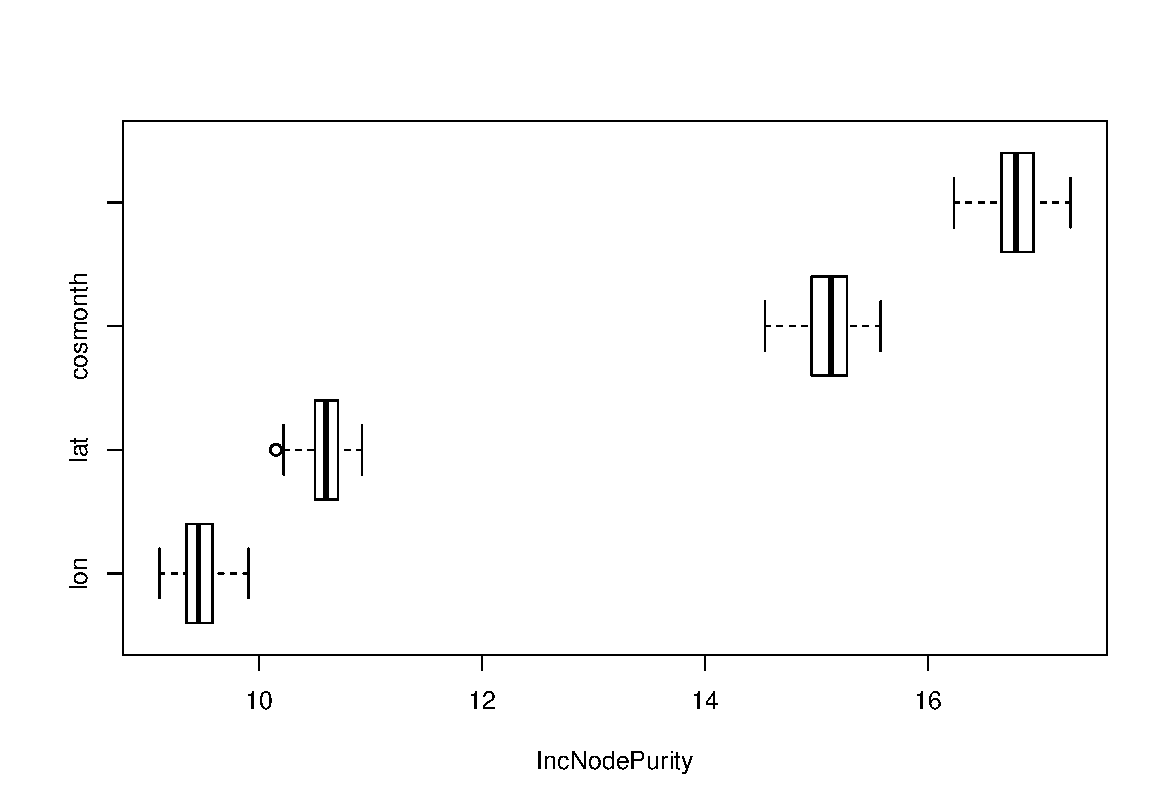
\includegraphics[scale=0.75]{VI.pdf}
		\caption{Example of variable importance plot of CQRF with \texttt{mtry=1} and \texttt{minnode=5}.}
		\label{fig:varimp}
	\end{figure}

	\subsection{Discussion}
	
	\section{Limitations and Further Works}
	
	The limitations of our alorithm are follows:
	
	First, circular transform is unique when we consider cosine and sine transformed value simultaneously. However, in this paper, traditional random forest algorithm do prediction parameter selection separately. We need to improve the algorithm.
	
	Second, it is known that the performance of random forest is better when the number of prediction variables is large. However, in this case, the number of predictor variables is small. 따라서 예측결과가 좋지 않을 수 있다.
	
	We need to develop quantile regression forests for an extreme quantile (Generalized random forest 및 extreme conditional quantile updgrade 버전 참고).

	\bibliographystyle{apalike}
	\bibliography{references}
\end{document}
